%%%%%%%%%%%%%%%%%%%%%%%%%%%%%%%%%%%%%%%%%%%%%%%%%%%%%%%%%%%%%%%%%%%%%%%%%%%%%%%%%%
\begin{frame}[fragile]\frametitle{}
\begin{center}
{\Large Regularizations}
\end{center}
\end{frame}

%%%%%%%%%%%%%%%%%%%%%%%%%%%%%%%%%%%%%%%%%%%%%%%%%%%%%%%%%%%%%%%%%%%%%%%%%%%%%%%%%%
\begin{frame}[fragile]\frametitle{The Problem}
Over-fitting

\begin{itemize}
\item Model built on training dataset works well, meaning, has less error.
\item Same model when used on the testing/validation set, then errors are more.
\item Reason: Over-fitting
\item Model has fitted the training data too rigidly, so that it does not work well on the other dataset, means, High Variance also.
\item Solution: to make model more generalized, less complex.
\item One such technique: Regularization
\item In regularization,normally we keep the same number of features, but reduce the magnitude of the coefficients. 
\item How does reducing the coefficients will help us?
\end{itemize}
\end{frame}

%%%%%%%%%%%%%%%%%%%%%%%%%%%%%%%%%%%%%%%%%%%%%%%%%%%%%%%%%%%%%%%%%%%%%%%%%%%%%%%%%%
\begin{frame}[fragile]\frametitle{Regularization}
\begin{itemize}
\item Example: Training data with x as weight and size as y.
\item We try to fit a line with minimum sum of squares. 
\item Say, we get the equation of the line
\item More the points better the general line.
\end{itemize}

\begin{center}
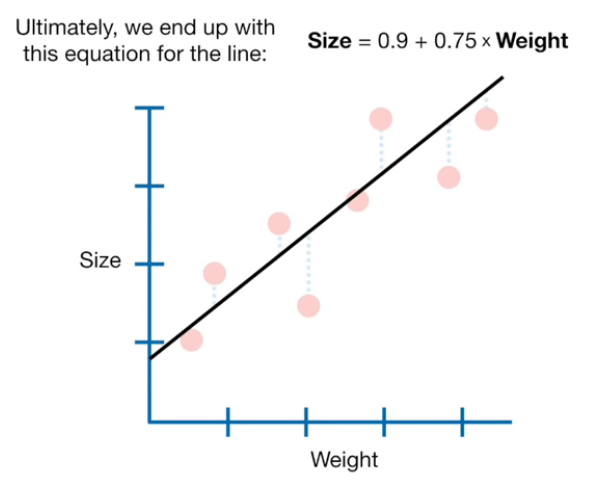
\includegraphics[width=0.5\linewidth,keepaspectratio]{regul1}
\end{center}

{\tiny (Ref: Regularization - StatQuest with Josh Stramer}
\end{frame}


%%%%%%%%%%%%%%%%%%%%%%%%%%%%%%%%%%%%%%%%%%%%%%%%%%%%%%%%%%%%%%%%%%%%%%%%%%%%%%%%%%
\begin{frame}[fragile]\frametitle{Regularization}
\begin{itemize}
\item But, say, we had very few points to train eg. only two!!
\item With Least Square method, we get the line, which obvously passes through both the points.
\item Whats the error while training?
\item Zero.
\item But what would be testing/validation (remaining points) error?
\item Large. High Variance, Over-fitting.
\end{itemize}

\begin{center}
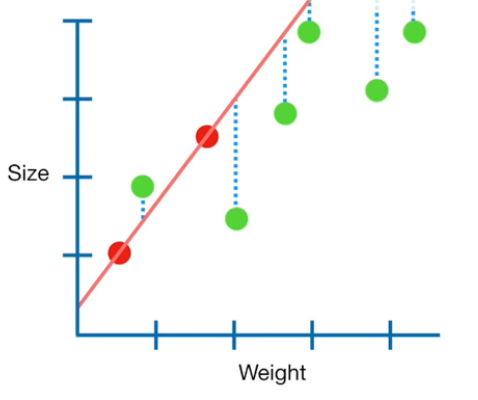
\includegraphics[width=0.4\linewidth,keepaspectratio]{regul2}
\end{center}

{\tiny (Ref: Regularization - StatQuest with Josh Stramer}
\end{frame}

%%%%%%%%%%%%%%%%%%%%%%%%%%%%%%%%%%%%%%%%%%%%%%%%%%%%%%%%%%%%%%%%%%%%%%%%%%%%%%%%%%
\begin{frame}[fragile]\frametitle{Regularization}
\begin{itemize}
\item Main idea behind Ridge Regression is NOT to fit the line perfectly!! 
\item So that variance with testing data is less.
\item This is done by adding small amount of BIAS in the LOSS equation. 
\item After Optimization, the Line shifts and thus the Variance reduces.
\end{itemize}

\begin{center}
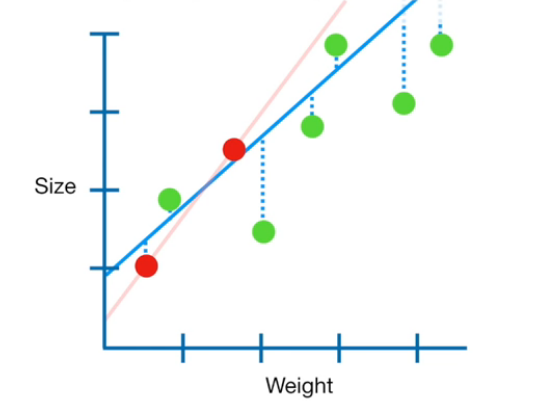
\includegraphics[width=0.5\linewidth,keepaspectratio]{regul3}
\end{center}

{\tiny (Ref: Regularization - StatQuest with Josh Stramer}
\end{frame}

%%%%%%%%%%%%%%%%%%%%%%%%%%%%%%%%%%%%%%%%%%%%%%%%%%%%%%%%%%%%%%%%%%%%%%%%%%%%%%%%%%
\begin{frame}[fragile]\frametitle{}
\begin{center}
{\Large Ridge Regression}
\end{center}
\end{frame}


%%%%%%%%%%%%%%%%%%%%%%%%%%%%%%%%%%%%%%%%%%%%%%%%%%%%%%%%%%%%%%%%%%%%%%%%%%%%%%%%%%
\begin{frame}[fragile]\frametitle{Ridge Regression}
\begin{itemize}
\item The Bias term is $\lambda \times slope^2$ (slope == weights or coefficients)
\item Example: Lets have some over-fitted line equation. 
\item As it passes through the point
\item In the Loss function, the sum of squares will be Zero, but the new bias term will have some value
\item Assume Lambda to be 1 for now, and the answer is 1.69. Meaning the Y intercept has SHIFTED!!.
\item The line does not pass through the two points any more, its more general, and thus avoids the over-fitting.
\end{itemize}

\begin{center}
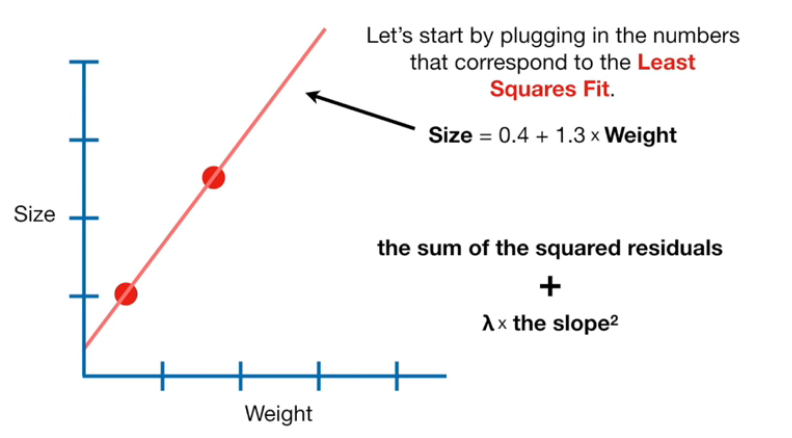
\includegraphics[width=0.5\linewidth,keepaspectratio]{regul4}
\end{center}

{\tiny (Ref: Regularization - StatQuest with Josh Stramer}
\end{frame}


%%%%%%%%%%%%%%%%%%%%%%%%%%%%%%%%%%%%%%%%%%%%%%%%%%%%%%%%%%%%%%%%%%%%%%%%%%%%%%%%%%
\begin{frame}[fragile]\frametitle{Ridge Regression}
\begin{itemize}
\item 1.69 is the Ridge Regression penalty.
\item If we optimize including the pentalty term, we will get new line, a new equation, say
 $Size = 0.9 + 0.8 \times Weight$ 
\item Its Ridge Regression penalty comes, say, 0.74, far less!! Better.
\end{itemize}

\begin{center}
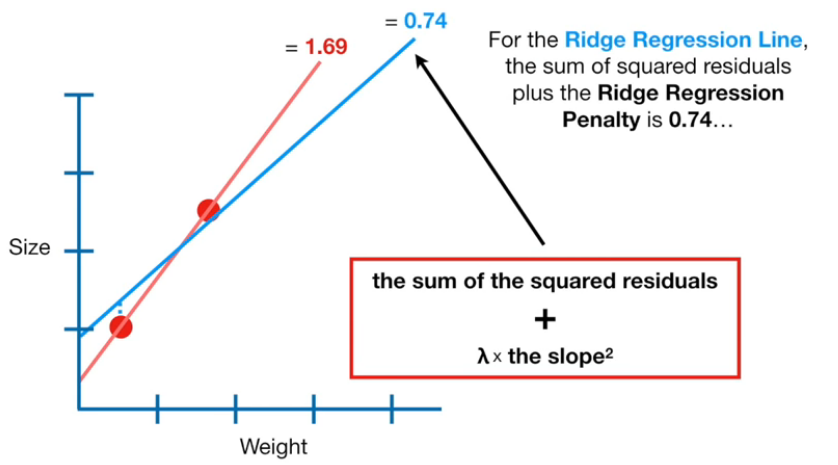
\includegraphics[width=0.8\linewidth,keepaspectratio]{regul5}
\end{center}

{\tiny (Ref: Regularization - StatQuest with Josh Stramer}
\end{frame}

%%%%%%%%%%%%%%%%%%%%%%%%%%%%%%%%%%%%%%%%%%%%%%%%%%%%%%%%%%%%%%%%%%%%%%%%%%%%%%%%%%
\begin{frame}[fragile]\frametitle{Ridge Regression}
\begin{itemize}
\item If the slope of the (original over-fit) line is steeper (meaning more weight value), meaning more y value change for same x change. More sensitive to small x change. 
\item Better to have smaller slope, for less sensitivity.
\item As seen before, due to Ridge regression, the slope got reduced.
\end{itemize}

\begin{center}
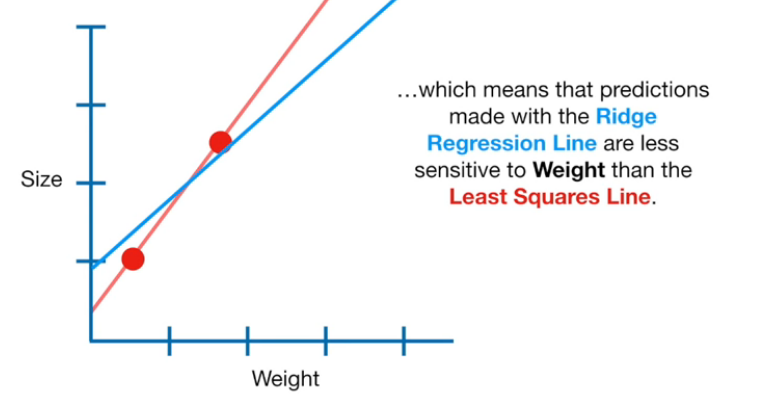
\includegraphics[width=0.8\linewidth,keepaspectratio]{regul6}
\end{center}

{\tiny (Ref: Regularization - StatQuest with Josh Stramer}
\end{frame}

%%%%%%%%%%%%%%%%%%%%%%%%%%%%%%%%%%%%%%%%%%%%%%%%%%%%%%%%%%%%%%%%%%%%%%%%%%%%%%%%%%
\begin{frame}[fragile]\frametitle{Ridge Regression}
\begin{itemize}
\item Minimization term in Ridge Regression line has the bias term also.
\item For $\lambda = 0$ the penalty term is 0 thus the line becomes same as Overfit line, which has 0 sum of squares error also.
\item But for Lambda values more than 0, it become flatter, with lambda as 2, more flatter, and so on.
\item We can try cross-validation and grid search to get good lambda value.
\item Ridge Regression penalty term has all the weight terms squared.
\end{itemize}

\begin{center}
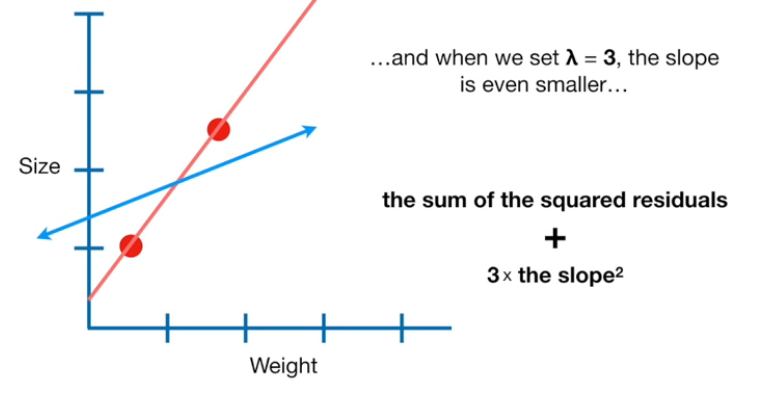
\includegraphics[width=0.8\linewidth,keepaspectratio]{regul7}
\end{center}

{\tiny (Ref: Regularization - StatQuest with Josh Stramer}
\end{frame}


%%%%%%%%%%%%%%%%%%%%%%%%%%%%%%%%%%%%%%%%%%%%%%%%%%%%%%%%%%%%%%%%%%%%%%%%%%%%%%%%%%
\begin{frame}[fragile]\frametitle{Sample Code}

\begin{lstlisting}
import matplotlib.pyplot as plt
import numpy as np 
import pandas as pd
import matplotlib
matplotlib.rcParams.update({'font.size': 12})
from sklearn.datasets import load_boston
from sklearn.cross_validation import train_test_split
from sklearn.linear_model import LinearRegression
from sklearn.linear_model import Ridge

boston=load_boston()
boston_df=pd.DataFrame(boston.data,columns=boston.feature_names)
boston_df['Price']=boston.target
newX=boston_df.drop('Price',axis=1)
print newX[0:3] # check 
newY=boston_df['Price']
\end{lstlisting}
\end{frame}

%%%%%%%%%%%%%%%%%%%%%%%%%%%%%%%%%%%%%%%%%%%%%%%%%%%%%%%%%%%%%%%%%%%%%%%%%%%%%%%%%%
\begin{frame}[fragile]\frametitle{Sample Code}

\begin{lstlisting}
X_train,X_test,y_train,y_test=train_test_split(newX,newY,test_size=0.3,random_state=3)

lr = LinearRegression()
lr.fit(X_train, y_train)

rr = Ridge(alpha=0.01) 
rr.fit(X_train, y_train)

rr100 = Ridge(alpha=100) #  comparison with alpha value
rr100.fit(X_train, y_train)
\end{lstlisting}

Higher the alpha value, more restriction on the coefficients; low alpha $>$ more generalization, coefficients are barely restricted and in this case linear and ridge regression resembles
\end{frame}



%%%%%%%%%%%%%%%%%%%%%%%%%%%%%%%%%%%%%%%%%%%%%%%%%%%%%%%%%%%%%%%%%%%%%%%%%%%%%%%%%%
\begin{frame}[fragile]\frametitle{Sample Code}

\begin{lstlisting}
train_score=lr.score(X_train, y_train)
test_score=lr.score(X_test, y_test)
Ridge_train_score = rr.score(X_train,y_train)
Ridge_test_score = rr.score(X_test, y_test)
Ridge_train_score100 = rr100.score(X_train,y_train)
Ridge_test_score100 = rr100.score(X_test, y_test)
print "linear regression train score:", train_score
print "linear regression test score:", test_score
print "ridge regression train score low alpha:", Ridge_train_score
print "ridge regression test score low alpha:", Ridge_test_score
print "ridge regression train score high alpha:", Ridge_train_score100
print "ridge regression test score high alpha:", Ridge_test_score100
\end{lstlisting}

\end{frame}


%%%%%%%%%%%%%%%%%%%%%%%%%%%%%%%%%%%%%%%%%%%%%%%%%%%%%%%%%%%%%%%%%%%%%%%%%%%%%%%%%%
\begin{frame}[fragile]\frametitle{Sample Code}

\begin{lstlisting}
plt.plot(rr.coef_,alpha=0.7,linestyle='none',marker='*',markersize=5,color='red',
label=r'Ridge; $\alpha = 0.01$',zorder=7) # zorder for ordering the markers

plt.plot(rr100.coef_,alpha=0.5,linestyle='none',marker='d',markersize=6,color='blue',
label=r'Ridge; $\alpha = 100$') # alpha here is for transparency

plt.plot(lr.coef_,alpha=0.4,linestyle='none',marker='o',markersize=7,color='green',
label='Linear Regression')

plt.xlabel('Coefficient Index',fontsize=16)
plt.ylabel('Coefficient Magnitude',fontsize=16)
plt.legend(fontsize=13,loc=4)
plt.show()
\end{lstlisting}

\end{frame}

%%%%%%%%%%%%%%%%%%%%%%%%%%%%%%%%%%%%%%%%%%%%%%%%%%%%%%%%%%%%%%%%%%%%%%%%%%%%%%%%%%
\begin{frame}[fragile]\frametitle{Ridge Regression}
\begin{itemize}
\item 13 features on x axis
\item For low value of $\alpha$, same as lambda (0.01), when the coefficients are less restricted, the magnitudes of the coefficients are almost same as of linear regression.
\item For higher value of $\alpha$ (100), we see that for coefficient indices 3,4,5 the magnitudes are considerably less compared to linear regression case. 
\end{itemize}

\begin{center}
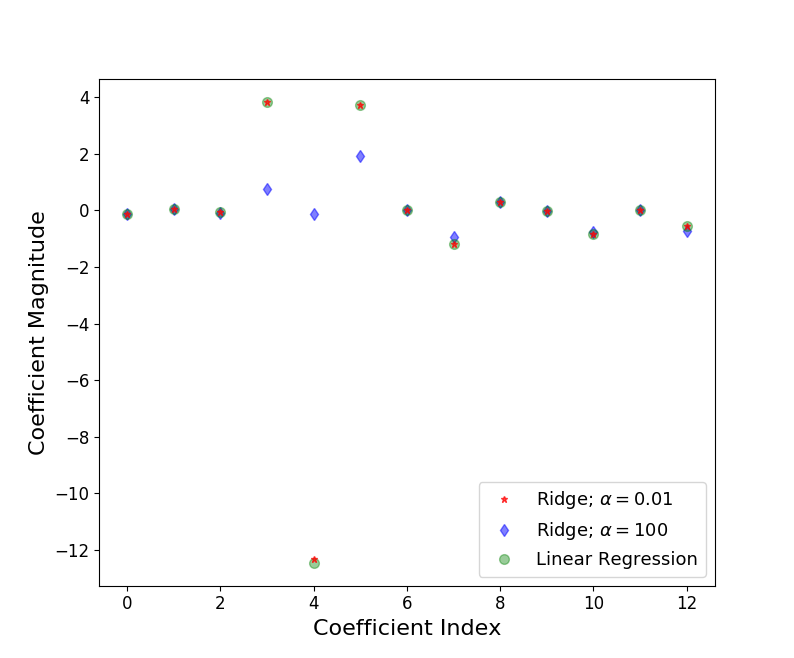
\includegraphics[width=0.5\linewidth,keepaspectratio]{regul8}
\end{center}

{\tiny (Ref: Ridge and Lasso Regression: A Complete Guide with Python Scikit-Learn - Saptashwa}
\end{frame}


% %%%%%%%%%%%%%%%%%%%%%%%%%%%%%%%%%%%%%%%%%%%%%%%%%%%%%%%%%%%%%%%%%%%%%%%%
% \begin{frame}[fragile]\frametitle{L2 Regularization (Ridge penalization| Gaussian Prior)}


	% \begin{itemize}
	% \item We can quantify complexity using the $L_2$ regularization formula, which defines the regularization term as the sum of the squares of all the feature weights: $L_2\text{ regularization term} = ||\boldsymbol w||_2^2 = {w_1^2 + w_2^2 + ... + w_n^2}$
	% \item In this formula, weights close to zero have little effect on model complexity, while outliers weights can have a huge impact.
	% \item Very large weights {\bf w} fit the training data very well, but poorly predict future data. 
	% \item ``Regularization'' means modifying the optimization problem to prefer small weights. 
	% \end{itemize}
	
	% % (Ref: https://developers.google.com/machine-learning/crash-course/regularization-for-simplicity/l2-regularization)
% \end{frame}

% %%%%%%%%%%%%%%%%%%%%%%%%%%%%%%%%%%%%%%%%%%%%%%%%%%%%%%%%%%%%%%%%%%%%%%%%
% \begin{frame}[fragile]\frametitle{Intuition}


	% \begin{itemize}
	% \item If you have two ways of fitting your data, such as $y=2x_1+0x_2$ or $y=x_1+x_2$, 
	% \item You prefer the latter because the penalty is $2^2+0^2=4$ in the former and $1^2+1^2=2$ in the latter. 
	% \item In general the effect of each weight on the prediction will be linear but its penalty will be quadratic. 
	% \item Thus it will pay off to put lots of small values instead of just a few big ones.
	% \end{itemize}
	
	% % (Ref: https://stats.stackexchange.com/questions/247940/how-does-the-l2-regularization-penalize-the-high-value-weights)
% \end{frame}

%%%%%%%%%%%%%%%%%%%%%%%%%%%%%%%%%%%%%%%%%%%%%%%%%%%%%%%%%%%%%%%%%%%%%%%%
\begin{frame}[fragile]\frametitle{Intuition}

\begin{center}
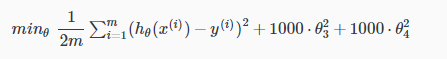
\includegraphics[width=0.7\linewidth,keepaspectratio]{reg4}
\end{center}

	\begin{itemize}
	\item Example: If we want to minimize the influence of two parameters, let's say $\theta_3$ and $\theta_4$, it seems like we have to give a large value of regularization parameter just like the equation below.
	

\item Why the bigger regularization parameter (lambda) reduces the influence instead of increasing it? How does this function work?

	\end{itemize}
	
	% (Ref: https://stackoverflow.com/questions/44742122/how-does-regularization-parameter-work-in-regularization)
\end{frame}

%%%%%%%%%%%%%%%%%%%%%%%%%%%%%%%%%%%%%%%%%%%%%%%%%%%%%%%%%%%%%%%%%%%%%%%%
\begin{frame}[fragile]\frametitle{Intuition}
\begin{center}
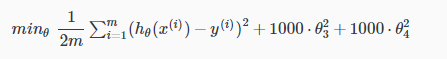
\includegraphics[width=0.7\linewidth,keepaspectratio]{reg4}
\end{center}

	\begin{itemize}
\item As you increase the regularization parameter, optimization function will have to choose a smaller theta in order to minimize the total cost.
\item In $L_2$ as thetas are enhanced by squaring, the reduction in their effect is more.
\item Its like feature selection by suppression of unwanted.
	\end{itemize}
	
	% (Ref: https://stackoverflow.com/questions/44742122/how-does-regularization-parameter-work-in-regularization)
\end{frame}



% %%%%%%%%%%%%%%%%%%%%%%%%%%%%%%%%%%%%%%%%%%%%%%%%%%%%%%%%%%%%%%%%%%%%%%%%
% \begin{frame}[fragile]\frametitle{Regularization}


	% \begin{itemize}
	% \item For example, a linear model with the following weights: $\{w_1 = 0.2, w_2 = 0.5, w_3 = 5, w_4 = 1, w_5 = 0.25, w_6 = 0.75\}$
	% \item Has an L2 regularization term of 26.915: $w_1^2 + w_2^2 + \boldsymbol{w_3^2} + w_4^2 + w_5^2 + w_6^2 = = 0.2^2 + 0.5^2 + \boldsymbol{5^2} + 1^2 + 0.25^2 + 0.75^2 = = 0.04 + 0.25 + \boldsymbol{25} + 1 + 0.0625 + 0.5625 = 26.915$
	% \item But $w_3$, with a squared value of 25, contributes nearly all the complexity. The sum of the squares of all five other weights adds just 1.915 to the L2 regularization term.
	% \end{itemize}
	
	% % (Ref: https://developers.google.com/machine-learning/crash-course/regularization-for-simplicity/l2-regularization)
% \end{frame}

% %%%%%%%%%%%%%%%%%%%%%%%%%%%%%%%%%%%%%%%%%%%%%%%%%%%%%%%%%%%%%%%%%%%%%%%%
% \begin{frame}[fragile]\frametitle{Regularization}


	% \begin{itemize}
	% \item Model developers tune the overall impact of the regularization term by multiplying its value by a scalar known as lambda (also called the regularization rate). That is, model developers aim to do the following: $minimize(Loss(Data|Model) + \lambda \text{ complexity(Model))}$
	% \item Lambda decides how much we care about the model fitting well versus how we care about  {\bf w} being small. 
	% \item Performing $L_2$ regularization has the following effect on a model
	% \begin{itemize}

		% \item Encourages weight values toward 0 (but not exactly 0) (near to 0 position)
		% \item Encourages the mean of the weights toward 0, with a normal (bell-shaped or Gaussian) distribution.
	% \end{itemize}
		% \end{itemize}

	% % (Ref: https://developers.google.com/machine-learning/crash-course/regularization-for-simplicity/l2-regularization)
% \end{frame}

% %%%%%%%%%%%%%%%%%%%%%%%%%%%%%%%%%%%%%%%%%%%%%%%%%%%%%%%%%%%%%%%%%%%%%%%%
% \begin{frame}[fragile]\frametitle{Regularization}
% Increasing the lambda value strengthens the regularization effect. For example, the histogram of a typical set of weights for a high value of lambda might look as shown below:

% \begin{center}
% 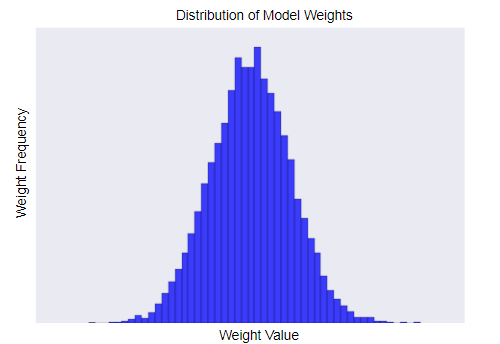
\includegraphics[width=0.6\linewidth,keepaspectratio]{reg2}
% \end{center}

	% % (Ref: https://developers.google.com/machine-learning/crash-course/regularization-for-simplicity/l2-regularization)
% \end{frame}

% %%%%%%%%%%%%%%%%%%%%%%%%%%%%%%%%%%%%%%%%%%%%%%%%%%%%%%%%%%%%%%%%%%%%%%%%
% \begin{frame}[fragile]\frametitle{Regularization}
% Lowering the value of lambda tends to yield a flatter histogram, as shown below:

% \begin{center}
% 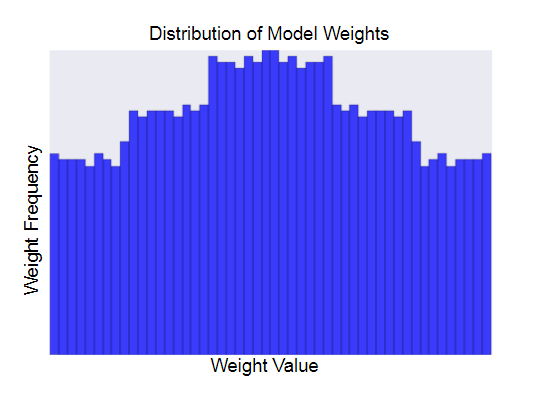
\includegraphics[width=0.6\linewidth,keepaspectratio]{reg3}
% \end{center}

	% % (Ref: https://developers.google.com/machine-learning/crash-course/regularization-for-simplicity/l2-regularization)
% \end{frame}

% %%%%%%%%%%%%%%%%%%%%%%%%%%%%%%%%%%%%%%%%%%%%%%%%%%%%%%%%%%%%%%%%%%%%%%%%
% \begin{frame}[fragile]\frametitle{Regularization}

% When choosing a lambda value, the goal is to strike the right balance between simplicity and training-data fit:
	% \begin{itemize}
	% \item If your lambda value is too high, your model will be simple, but you run the risk of under-fitting your data. Your model won't learn enough about the training data to make useful predictions.

% \item If your lambda value is too low, your model will be more complex, and you run the risk of over-fitting your data. Your model will learn too much about the particularities of the training data, and won't be able to generalize to new data.
		% \end{itemize}

	% % (Ref: https://developers.google.com/machine-learning/crash-course/regularization-for-simplicity/l2-regularization)
% \end{frame}

%%%%%%%%%%%%%%%%%%%%%%%%%%%%%%%%%%%%%%%%%%%%%%%%%%%%%%%%%%%%%%%%%%%%%%%%%%%%%%%%%%
\begin{frame}[fragile]\frametitle{}
\begin{center}
{\Large Lasso Regression}
\end{center}
\end{frame}

%%%%%%%%%%%%%%%%%%%%%%%%%%%%%%%%%%%%%%%%%%%%%%%%%%%%%%%%%%%%%%%%%%%%%%%%%%%%%%%%%%
\begin{frame}[fragile]\frametitle{Lasso Regression}
\begin{itemize}
\item Ridge Regression penalty is $\lambda \sum{weights^2}$
\item For Lasso Regression the penalty is $\lambda \sum{|weights|}$
\item Similarly, due to added bias, the line flattens a bit.
\item 
\end{itemize}

\begin{center}
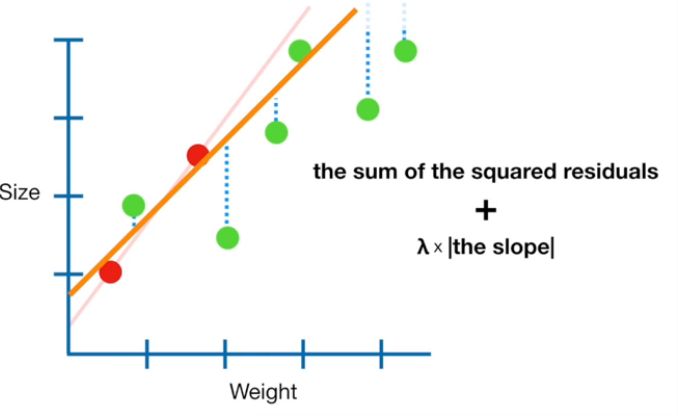
\includegraphics[width=0.8\linewidth,keepaspectratio]{regul9}
\end{center}

{\tiny (Ref: Regularization - StatQuest with Josh Stramer}
\end{frame}


%%%%%%%%%%%%%%%%%%%%%%%%%%%%%%%%%%%%%%%%%%%%%%%%%%%%%%%%%%%%%%%%%%%%%%%%%%%%%%%%%%
\begin{frame}[fragile]\frametitle{Similarity}
Both Ridge and Lasso have similar looking formula, and they behave similarly ie they flatten the over-fit line. 


\begin{center}
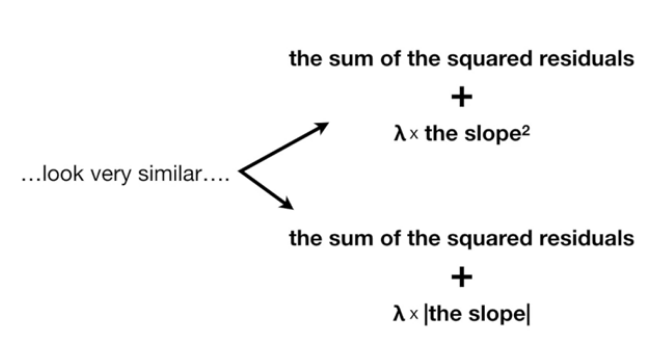
\includegraphics[width=0.8\linewidth,keepaspectratio]{regul10}
\end{center}

{\tiny (Ref: Regularization - StatQuest with Josh Stramer}
\end{frame}

%%%%%%%%%%%%%%%%%%%%%%%%%%%%%%%%%%%%%%%%%%%%%%%%%%%%%%%%%%%%%%%%%%%%%%%%%%%%%%%%%%
\begin{frame}[fragile]\frametitle{Difference}
As lambda increase slope can turn to 0 (not just TENDS to 0 as in Ridge Regression).
That means it eliminates useless features completely.

\begin{center}
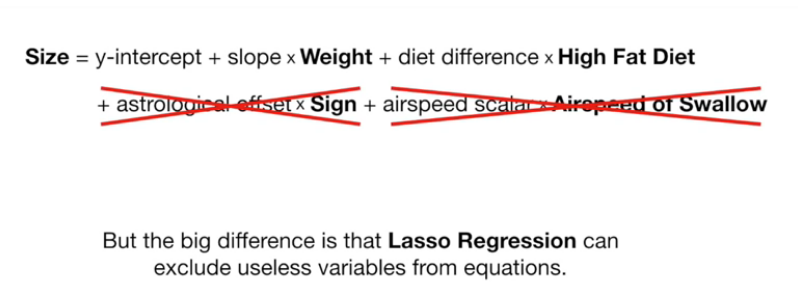
\includegraphics[width=0.8\linewidth,keepaspectratio]{regul12}
\end{center}

{\tiny (Ref: Regularization - StatQuest with Josh Stramer}
\end{frame}



%%%%%%%%%%%%%%%%%%%%%%%%%%%%%%%%%%%%%%%%%%%%%%%%%%%%%%%%%%%%%%%%%%%%%%%%%%%%%%%%%%
\begin{frame}[fragile]\frametitle{Sample Code}

\begin{lstlisting}
import matplotlib.pyplot as plt
import numpy as np 
import pandas as pd
import matplotlib
from sklearn.linear_model import Lasso
from sklearn.linear_model import LinearRegression
from sklearn.datasets import load_breast_cancer
from sklearn.cross_validation import train_test_split

cancer = load_breast_cancer()
cancer_df = pd.DataFrame(cancer.data, columns=cancer.feature_names)
X = cancer.data
Y = cancer.target
\end{lstlisting}
\end{frame}

%%%%%%%%%%%%%%%%%%%%%%%%%%%%%%%%%%%%%%%%%%%%%%%%%%%%%%%%%%%%%%%%%%%%%%%%%%%%%%%%%%
\begin{frame}[fragile]\frametitle{Sample Code}

\begin{lstlisting}
X_train,X_test,y_train,y_test=train_test_split(X,Y, test_size=0.3, random_state=31)

lasso = Lasso()
lasso.fit(X_train,y_train)
train_score=lasso.score(X_train,y_train)
test_score=lasso.score(X_test,y_test)
coeff_used = np.sum(lasso.coef_!=0)
print "training score:", train_score 
print "test score: ", test_score
print "number of features used: ", coeff_used
\end{lstlisting}


\end{frame}



%%%%%%%%%%%%%%%%%%%%%%%%%%%%%%%%%%%%%%%%%%%%%%%%%%%%%%%%%%%%%%%%%%%%%%%%%%%%%%%%%%
\begin{frame}[fragile]\frametitle{Sample Code}

\begin{lstlisting}
lasso001 = Lasso(alpha=0.01, max_iter=10e5)
lasso001.fit(X_train,y_train)
train_score001=lasso001.score(X_train,y_train)
test_score001=lasso001.score(X_test,y_test)
coeff_used001 = np.sum(lasso001.coef_!=0)
print "training score for alpha=0.01:", train_score001 
print "test score for alpha =0.01: ", test_score001
print "number of features used: for alpha =0.01:", coeff_used001
\end{lstlisting}

\end{frame}


%%%%%%%%%%%%%%%%%%%%%%%%%%%%%%%%%%%%%%%%%%%%%%%%%%%%%%%%%%%%%%%%%%%%%%%%%%%%%%%%%%
\begin{frame}[fragile]\frametitle{Sample Code}

\begin{lstlisting}
lasso00001 = Lasso(alpha=0.0001, max_iter=10e5)
lasso00001.fit(X_train,y_train)
train_score00001=lasso00001.score(X_train,y_train)
test_score00001=lasso00001.score(X_test,y_test)
coeff_used00001 = np.sum(lasso00001.coef_!=0)
print "training score for alpha=0.0001:", train_score00001 
print "test score for alpha =0.0001: ", test_score00001
print "number of features used: for alpha =0.0001:", coeff_used00001
\end{lstlisting}

\end{frame}

%%%%%%%%%%%%%%%%%%%%%%%%%%%%%%%%%%%%%%%%%%%%%%%%%%%%%%%%%%%%%%%%%%%%%%%%%%%%%%%%%%
\begin{frame}[fragile]\frametitle{Sample Code}

\begin{lstlisting}
lr = LinearRegression()
lr.fit(X_train,y_train)
lr_train_score=lr.score(X_train,y_train)
lr_test_score=lr.score(X_test,y_test)
print "LR training score:", lr_train_score 
print "LR test score: ", lr_test_score
\end{lstlisting}

\end{frame}


%%%%%%%%%%%%%%%%%%%%%%%%%%%%%%%%%%%%%%%%%%%%%%%%%%%%%%%%%%%%%%%%%%%%%%%%%%%%%%%%%%
\begin{frame}[fragile]\frametitle{Sample Code}
Output

\begin{lstlisting}
training score: 0.5600974529893081
test score:  0.5832244618818156
number of features used:  4
training score for alpha=0.01: 0.7037865778498829
test score for alpha =0.01:  0.664183157772623
number of features used: for alpha =0.01: 10
training score for alpha=0.0001: 0.7754092006936697
test score for alpha =0.0001:  0.7318608210757904
number of features used: for alpha =0.0001: 22
LR training score: 0.7842206194055068
LR test score:  0.7329325010888681
\end{lstlisting}

\end{frame}

%%%%%%%%%%%%%%%%%%%%%%%%%%%%%%%%%%%%%%%%%%%%%%%%%%%%%%%%%%%%%%%%%%%%%%%%%%%%%%%%%%
\begin{frame}[fragile]\frametitle{Sample Code}

\begin{lstlisting}
plt.subplot(1,2,1)
plt.plot(lasso.coef_,alpha=0.7,linestyle='none',marker='*',markersize=5,
color='red',label=r'Lasso; $\alpha = 1$',zorder=7) # alpha here is for transparency

plt.plot(lasso001.coef_,alpha=0.5,linestyle='none',marker='d',markersize=6,
color='blue',label=r'Lasso; $\alpha = 0.01$') # alpha here is for transparency

plt.xlabel('Coefficient Index',fontsize=16)
plt.ylabel('Coefficient Magnitude',fontsize=16)
plt.legend(fontsize=13,loc=4)
\end{lstlisting}

\end{frame}

%%%%%%%%%%%%%%%%%%%%%%%%%%%%%%%%%%%%%%%%%%%%%%%%%%%%%%%%%%%%%%%%%%%%%%%%%%%%%%%%%%
\begin{frame}[fragile]\frametitle{Sample Code}

\begin{lstlisting}
plt.subplot(1,2,2)
plt.plot(lasso.coef_,alpha=0.7,linestyle='none',marker='*',markersize=5,
color='red',label=r'Lasso; $\alpha = 1$',zorder=7) # alpha here is for transparency

plt.plot(lasso001.coef_,alpha=0.5,linestyle='none',marker='d',markersize=6,
color='blue',label=r'Lasso; $\alpha = 0.01$') # alpha here is for transparency

plt.plot(lasso00001.coef_,alpha=0.8,linestyle='none',marker='v',markersize=6,
color='black',label=r'Lasso; $\alpha = 0.00001$') # alpha here is for transparency

plt.plot(lr.coef_,alpha=0.7,linestyle='none',marker='o',markersize=5,
color='green',label='Linear Regression',zorder=2)

plt.xlabel('Coefficient Index',fontsize=16)
plt.ylabel('Coefficient Magnitude',fontsize=16)
plt.legend(fontsize=13,loc=4)
plt.tight_layout()
plt.show()
\end{lstlisting}

\end{frame}




%%%%%%%%%%%%%%%%%%%%%%%%%%%%%%%%%%%%%%%%%%%%%%%%%%%%%%%%%%%%%%%%%%%%%%%%%%%%%%%%%%
\begin{frame}[fragile]\frametitle{Lasso Regression}

\begin{center}
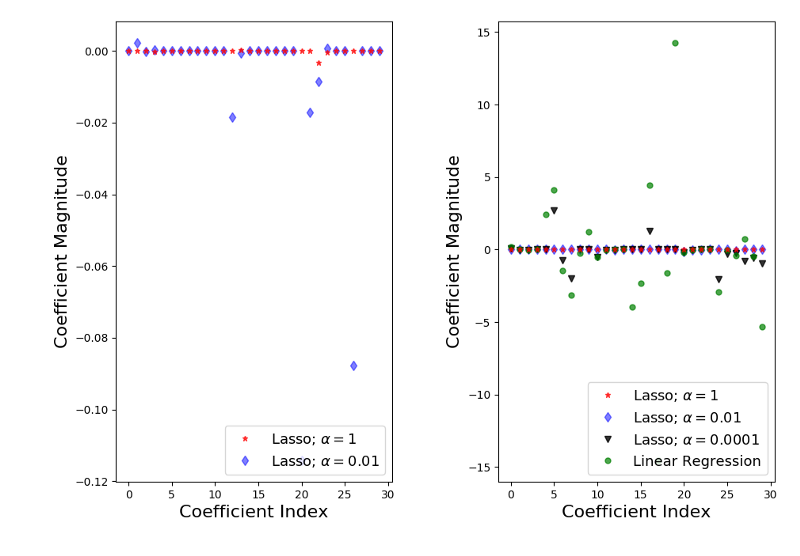
\includegraphics[width=0.8\linewidth,keepaspectratio]{regul11}
\end{center}

{\tiny (Ref: Ridge and Lasso Regression: A Complete Guide with Python Scikit-Learn - Saptashwa}
\end{frame}


%%%%%%%%%%%%%%%%%%%%%%%%%%%%%%%%%%%%%%%%%%%%%%%%%%%%%%%%%%%%%%%%%%%%%%%%%%%%%%%%%%
\begin{frame}[fragile]\frametitle{Lasso Regression}
\begin{itemize}
\item With this, out of 30 features in cancer data-set, only 4 features are used (non zero value of the coefficient).
\item Both training and test score (with only 4 features) are low; conclude that the model is under-fitting the cancer data-set.
\item Reduce this under-fitting by reducing alpha and increasing number of iterations. Now $\alpha = 0.01$, non-zero features =10, training and test score increases.
\item Comparison of coefficient magnitude for two different values of alpha are shown in the left panel of figure 2. For alpha =1, we can see most of the coefficients are zero or nearly zero, which is not the case for alpha=0.01.
\item Further reduce $\alpha =0.0001$, non-zero features = 22. Training and test scores are similar to basic linear regression case.
\item In the right panel of figure, for $\alpha = 0.0001$, coefficients for Lasso regression and linear regression show close resemblance.
\end{itemize}


{\tiny (Ref: Ridge and Lasso Regression: A Complete Guide with Python Scikit-Learn - Saptashwa}
\end{frame}




%%%%%%%%%%%%%%%%%%%%%%%%%%%%%%%%%%%%%%%%%%%%%%%%%%%%%%%%%%%%%%%%%%%%%%%%%%%%%%%%%%%%%%%%%%%%

% %https://darrenho.github.io/SML2015/linearModelRegularization.tex

% \begin{frame}[fragile]
% \frametitle{Least squares}

% % \begin{figure}[!h]
% % \includegraphics[width=3in,trim=0 40 0 0,clip]{../figures/3dSquaredErrorOnly.pdf}
% % \end{figure}
% $\beta_{LS} = argmin { \beta\in\mathbb{R}^p} ||Y - X  \beta||_2^2$
% \end{frame}



% \begin{frame}[fragile]
% \frametitle{Regularization}
% Another way to control bias and variance is through {regularization} or
% {shrinkage}.  


% The idea is to make your
% estimates of $\beta$ `smaller', rather than set them to zero 

% {\scriptsize (which is what all subsets does)}


% One way to do this is called {ridge regression}\footnote{Hoerl, Kennard  (1970)}:
% $
% \beta{t} = argmin { || \beta ||_2^2 \leq t} ||Y - X  \beta||_2^2
% $
% for any $t \geq 0$.  




% Compare this to {least squares}

% $
% \beta_{LS} = argmin { \beta\in\mathbb{R}^p} ||Y - X  \beta||_2^2
% $

% \end{frame}



% % \begin{frame}
% % \frametitle{Geometry of ridge regression in $\mathbb{R}^2$}
% % \begin{figure}
  % % \centering
   % % \includegraphics[width=2in,trim=40 50 40 50,clip] {../figures/l_pBalls2ellipseAnnotated.pdf} 
   % % \includegraphics[width=2in,trim=0 0 0 0,clip]{../figures/3dSquaredErrorOnly.pdf}
% % \end{figure}
% % \end{frame}  

% \begin{frame}[fragile]
% \frametitle{Ridge regression}
% An equivalent way to write
% \begin{equation}
% \beta{t} = argmin { || \beta ||_2^2 \leq t} ||Y - X  \beta||_2^2
% \label{eq:1}
% \end{equation}
% is in the {Lagrangian} form
% \begin{equation}
% \beta{\lambda} = argmin { \beta} ||Y - X  \beta||_2^2 + \lambda || \beta ||_2^2.
% \label{eq:2}
% \end{equation}
% For every $\lambda'$ there is a unique $t'$ (and vice versa) that makes 
% $
% \beta{\lambda'} = \beta{t'}
% $
% \end{frame}

% \begin{frame}[fragile]
% \frametitle{Regularization and standardization}
% The coefficient vector isn't invariant to rescaling. 


% If an intercept is included, do not penalize it:
% $
% \min_{\beta_0,\beta} \sum_{i=1}^n (Y_i - \beta_0 + \beta^{\top}X_i)^2 + \lambda norm{\beta}_2^2
% $

% The usual way of addressing this in regression is:
% \begin{itemize}
% \item {Standardize} {all} covariates for which scale is meaningful:
% $
% x_j \leftarrow \frac{(x_j - \textrm{mean}(x_j))}{\textrm{sd}(x_j)}
% $

% {So, don't standardize indictor variables, for instance }
% \item Standardize the response $Y \leftarrow Y - \textrm{mean}(Y)$
% \item Don't include an intercept

% {It would have been equal to $\textrm{mean}(Y)$}
% \end{itemize}
% \end{frame}

% \begin{frame}[fragile]
% \frametitle{Ridge regression}

% Observe:
% \begin{itemize}
% \item $\lambda = 0$ (or $t = \infty$) makes $\beta{\lambda = 0} = \beta_{LS}$
% \item Any $\lambda > 0$ (or $t <\infty$)  penalizes larger values of $ \beta$, effectively shrinking them.
% \end{itemize}

% Note: $\lambda$ and $t$ are known as {tuning parameters} 

% {Alternatively, hyper-parameters}


% However we think about it, we have produced a {suite} of solutions
% $
% \{\beta{\lambda} : \lambda \in [0,\infty)\}
% $
% What do these solutions look like?

% \end{frame}

% % \begin{frame}
% % \frametitle{Ridge regression path}
% % \begin{figure}
  % % \centering
   % % \includegraphics[width=3in] {../figures/beta_ridgePathNoCV.pdf} 
% % \end{figure}
% % \end{frame}  

% \begin{frame}
% \frametitle{Ridge regression}
% {Reminder:} The least squares solution can be written:
% $
% \hat\beta_{\textrm{LS}} = (X^{\top} X)^{\dagger} X^{\top} Y.
% $

% However, if $rank(X) < p$, then $\hat\beta_{\textrm{LS}}$ is not unique.  In fact, 
% $
% \forall b \in \{b:X b = 0\} 
% $
 % $\hat\beta_{\textrm{LS}} + b$ is a valid least squares solution.  


% It turns out through differential calculus, we can write out the ridge regression solution as well:
% $
% \beta{\lambda} = (X^{\top} X + \lambda I)^{-1} X^{\top} Y 
% $

% Quite similar.  However, the $\lambda$ can make all the difference..
% \end{frame}


% \begin{frame}
% \frametitle{Regularization - Ridge Regression}

% Using the {SVD} $(X = U D V^{\top})$, we can look even deeper. 
% \begin{align*}
% \beta_{\textrm{LS}} & = V D^{-1} U^{\top} Y  & = & \sum_{j=1}^p v_j \left(\frac{1}{d_j} \right)u_j^{\top}Y \\
% \beta{\lambda} & = V (D^2 + \lambda I)^{-1} D U^{\top} Y & = & \sum_{j=1}^p v_j \left( \frac{d_j}{d_j^2 + \lambda} \right)u_j^{\top}Y.
% \end{align*}
% Similarly
% \begin{align*}
% X\beta_{\textrm{LS}} & = U U^{\top} Y  & = & \sum_{j=1}^p u_j u_j^{\top}Y \\
% X\beta{\lambda} & = U D (D^2 + \lambda I)^{-1} D U^{\top} Y & = & \sum_{j=1}^p u_j \left( \frac{d_j^2}{d_j^2 + \lambda} \right)u_j^{\top}Y.
% \end{align*}

% \textbf{$\Rightarrow$ Ridge shrinks the data by an additional factor of $\lambda$}.
% \end{frame}


% \begin{frame}[fragile]
% \frametitle{Ridge Regression: A Bayesian approach }
% Suppose we specify the likelihood as
% $
% Y_i \sim N(X_i^{\top}\beta, \sigma^2)
% $
% and put a prior distribution of $\beta \sim N(0,\tau^2I)$.


% Then we have the following posterior (making some conditional independence assumptions)
% $
% p(\beta | Y, X, \sigma^2,\tau^2) \propto p(Y | X ,\beta, \sigma^2) p(\beta | \tau^2).
% $
% After kernel matching, we find that the posterior mode/mean is
% $
% \beta{\lambda = \sigma^2/\tau^2}
% $
% \end{frame}


% \begin{frame}
% \frametitle{Ridge regression in a new space }
% Note the matrix identity
% $
% (A - BC^{-1}E)^{-1}BC^{-1} = A^{-1} B (C -  EA^{-1}B)^{-1}
% $
% {Henderson, Searle (1980), equation (13)}

% Then,
% $
% \beta{\lambda} = (X^{\top} X + \lambda I)^{-1} X^{\top} Y = X^{\top}( XX^{\top} + \lambda I)^{-1}Y
% $
% \end{frame}

% \begin{frame}
% \frametitle{Ridge  in a new space: Computations }
% The ridge solution solves either the {normal equations}
% $
% (X^{\top} X + \lambda I)\hat\beta =  X^{\top} Y 
% $
% or the {adjoint problem}
% $
% X^{\top}( XX^{\top} + \lambda I)^{-1}Y
% $
% The `heavy lifting' in each case is done with the inversion


% \begin{itemize}
% \item $X^{\top} X \in R^{p \times p} \Longrightarrow$ takes $p^3$ computations, $p^2$ space 
% \item $ X X^{\top}\in R^{n \times n} \Longrightarrow$ takes $n^3$ computations, $n^2$ space
% \end{itemize}

% {Conclusion:} Depending on the relative size of $n$ and $p$, this could be substantial
% savings


% However, a much deeper realization is possible..
% \end{frame}



% \begin{frame}
% \frametitle{(Kernel) ridge regression}
% Suppose we want to predict at $X$, then 
% $
% \hat{f}(X) = X^{\top}\beta{\lambda} =  X^{\top}X^{\top}( XX^{\top} + \lambda I)^{-1}Y
% $
% Also,
% $
% XX^{\top} = 
% \begin{bmatrix}
% \langle X_1, X_1 Rangle & \langle X_1, X_2 Rangle & \cdots & \langle X_1, X_n Rangle \\
% & vdots && \\
% \langle X_n, X_1 Rangle & \langle X_n, X_2 Rangle & \cdots & \langle X_n, X_n Rangle
% \end{bmatrix}
% $
% and
% $
% X^{\top}X^{\top} = [\langle X, X_1 Rangle,  \langle X, X_2 Rangle, \cdots, \langle X, X_n Rangle]
% $
% where $\langle X,X' Rangle = X^{\top}X'$ is the Euclidean inner product.


% If we transform $X_i \mapsto \Phi(X_i)$, and the range of $\Phi$ is equipped with an inner product, we can use
% $\langle \Phi(X_i), \Phi(X_{i'}) Rangle$


% Inserting $\Phi$ is known as {kernelization} or a {kernel trick}
% \end{frame}


% \begin{frame}
% \frametitle{(Kernel) ridge regression}
% {Example:} Suppose $X = (\textrm{income},\textrm{height})^{\top}$

 % Then we could specify the map 
% $
% \Phi(X)^{\top} = (\textrm{income},\textrm{height}, \textrm{income}*\textrm{height},\textrm{income}^2,\textrm{height}^2)
% $
% The induced {feature matrix} is then
% $
% X = 
% \begin{bmatrix}
% \Phi(X_1) \\
 % vdots  \\
% \Phi(X_n)
% \end{bmatrix}
% \in
% R^{n \times 5}
% $
% \end{frame}

% \begin{frame}
% \frametitle{(Kernel) ridge regression}
% Ordinarily, this would mean we need to solve the {normal equation} inversion for $p = 5$
% \begin{itemize}
% \item $X^{\top} X \in R^{p \times p} \Longrightarrow$ takes $p^3$ computations, $p^2$ space 
% \end{itemize}


% However, using the {kernel trick} we can solve instead
% \begin{itemize}
% \item $ X X^{\top}\in R^{n \times n} \Longrightarrow$ takes $n^3$ computations, $n^2$ space
% \end{itemize}
% which is fixed in $p$

% vvvsp
% {Implication:} We can add essentially arbitrary nonlinearity without paying higher computational, storage
 % cost!
 
 % vvsp
 % We will return to this again with {support vector machines} (SVM)
% \end{frame}

% % \transitionSlide{Ridge in practice}

% % \begin{frame}[fragile]
% % \frametitle{Ridge Regression: The tuning parameter}
% % We can use a degrees of freedom based risk estimator to choose $\lambda$


% % The degrees of freedom of $\beta{\lambda}$ can be seen to be
% % $
% % \df = \tr \left[X(X^{\top}X + \lambda I)^{-1} X^{\top}Right] = \sum_{j=1}^p \frac{d_j^2}{d_j^2 + \lambda}
% % $
% % {As $\lambda Rightarrow 0$, we get the number of parameters}

% % A common, classic choice is {generalized cross-validation} (GCV), which has the form:
% % $
% % \textrm{GCV}(\hat\beta) = \frac{\hat\P \ell_{\hat{\beta}}}{(1-\df(\hat{\beta})/n)^2}
% % $

% % {Golub, Heath, Wahba (1979)}


% % Note that this looks a lot like AIC with unknown variance, but with $\log(1- \df{}/n)$ as penalty
% % \end{frame}

% % \begin{frame}[fragile]
% % \frametitle{Ridge Regression: The tuning parameter}
% % To see this last claim, observe

% % \begin{align*}
% % \log\left(\textrm{GCV}(\hat\beta)Right) &\propto \log(\train) - 2\log(1-\df(\hat{\beta})/n)\\
% % \textrm{{versus}} & \\
% % \textrm{AIC}(\hat\beta) & \propto \log(\train) +  2n^{-1}\df(\hat{\beta})
% % \end{align*}

% % \end{frame}

% % \begin{frame}[fragile]
% % \frametitle{Ridge Regression: The tuning parameter}
% % Nowadays, using $K$-fold cross-validation is common


% % Think of $CV_K$ as a function of $\lambda$, and pick its {minimum}:
% % $
% % \hat\lambda = argmin {\lambda \geq 0} CV_K(\lambda)
% % $


% % Now, we report $\beta{\hat\lambda}$ as our estimator
% % \end{frame}


% % \begin{frame}[fragile]
% % \frametitle{Ridge Regression: Computation}
% % There are several ways to compute ridge regression


% % We can follow any conventional least squares solving technique (i.e.: QR factorization, Cholesky Decomposition, SVD,...):
% % $
% % (X^{\top}X + \lambda I)\beta = X^{\top}Y
% % $


% % Alternatively, we can actually solve it using \alr{lm} in \alr{R} if we make the following augmentation

% % $
% % \tilde{Y} = 
% % \begin{bmatrix}
% % Y_1 \\
% % vdots \\
% % Y_n \\
% % 0 \\
% % vdots \\
% % 0
% % \end{bmatrix}
% % \in
% % R^{n + p}
% % \textrm{ and }
% % \tilde{X} = 
% % \begin{bmatrix}
% % X \\
% % \sqrt{\lambda} I 
% % \end{bmatrix}
% % $
% % \end{frame}

% % \begin{frame}[fragile]
% % \frametitle{Ridge Regression in R}

% % We will concentrate on a slightly more complicated way, as it will make  things easier later.

% % \begin{blockcode}
% % install.packages('glmnet')
% % library(glmnet)
% % ridge.out = cv.glmnet(x=X,y=Y,alpha=0)
% % \end{blockcode}

% % \end{frame}

% % \begin{frame}[fragile]
% % \frametitle{Ridge Regression: CV plot}
% % \begin{blockcode}
% % X = as.matrix(X)
% % ridge.out = cv.glmnet(x=X,y=Y,alpha=0)

% % plot(ridge.out$lambda,ridge.out$cvm,
       % % xlab='lambda',ylab='CV error',main='Ridge',type='l')
% % abline(v=ridge.out$lambda[which.min(ridge.out$cvm)])
% % \end{blockcode}
% % %min.lambda = min(ridge.out$lambda)
% % %lambda.new = seq(min.lambda*10,min.lambda*.001,length=100)
% % %ridge.out = cv.glmnet(x=X,y=Y,alpha=0,lambda=lambda.new)

% % \begin{figure}
  % % \centering 
  % % \includegraphics[width=1.6in,trim=0 0 0 25,clip] {../figures/ridgeCV} 
% % \end{figure}    

% % \end{frame}

% % \begin{frame}
% % \frametitle{Ridge regression path}
% % \begin{figure}
  % % \centering
   % % \includegraphics[width=3in] {../figures/beta_ridgePath.pdf} 
% % \end{figure}
% % \end{frame}  


% %\begin{frame}[fragile]
% %\frametitle{Ridge Regression: Using the $\lambda$}
% %Here is the chosen fit (along with some previous methods):
% %\begin{blockcode}
% %#for predictor coefficient estimates
% %ridge.out$glmnet.fit$beta[,which.min(ridge.out$cvm)] 
% %#for intercept
% %ridge.out$glmnet.fit$a0[which.min(ridge.out$cvm)] 
% %\end{blockcode}
% %\begin{tabular}{lrrr}
% %Variable & Ridge & Full Linear Model & Forward and Backward\\ 
% %%intercept & -0.017  & 0.181561 &  0.4947\\
% %lcavol   &  0.474  &  0.564341  & 0.543 \\
% %lweight  &   0.597 &  0.622020 & 0.588\\
% %age &  -0.015 &   -0.021248  & -0.016 \\
% %lbph & 0.083   & 0.096713 & 0.101\\
% %svi & 0.667  & 0.761673 & 0.715 \\
% %lcp &  -0.025 & -0.106051 & 0\\
% %gleason & 0.066 & 0.049228 & 0  \\
% %pgg45 &  0.003 & 0.004458 & 0\\
% %\end{tabular}
% %\end{frame}
% %
% %\begin{frame}[fragile]
% %\frametitle{Ridge regression and multicollinearity}
% %Multicollinearity is a phenomenon in which a combination of predictor variables is extremely similar to
% %another predictor variable. Some comments:
% %\begin{itemize}
% %\item A better term that is sometimes used is {$X$ is ill-conditioned}
% %\item It means that one of its columns is nearly (or exactly) a linear combination of other columns.  This is sometimes known
% %as `(numerically) rank-deficient'.
% %\item If $X = U D V^{\top}$ is ill-conditioned, then some elements of $D$ are {nearly zero} 
% %
% %{size (remember, $D$ is a diagonal matrix with decreasing entries)}
% %\item If we form $\beta_{LS} = (X^{\top}X)^{-1}X^{\top}Y = V D^{-1} U^{\top} Y$, then we see that the small
% %entries of $D$ are now huge (due to the inverse).  This in turn creates a {huge variance }
% %
% %{size ($\mathbb{V} \beta_{LS} =  (X^{\top}X)^{-1} = V D^{-2} V^{\top}$)}
% %\end{itemize}
% %\end{frame}
% %
% %\begin{frame}[fragile]
% %\frametitle{Ridge regression and multicollinearity}
% %Ridge Regression fixes this problem by preventing the division by a {near zero number}  
% %
% %vsp
% %\emphasis{9cm}{Example:}{If $a$ is a really small number, and $\lambda > 0$ is another number, then
% %\[
% %\frac{1}{a} \approx \infty \quad \textrm{while} \quad \frac{1}{a + \lambda} \textrm{ is much smaller.}
% %\]
% %To wit, $1/0.0001 = 10,000$, while $1/(0.0001 + 0.1) \approx 10$}
% %
% %vsp
% %
% %\emphasis{7cm}{Conclusion:}{
% %
% %$(X^{\top}X)^{-1}$ can be really unstable, while $(X^{\top}X + \lambda I)^{-1}$ is not.}
% %\end{frame}
% %
% %\begin{frame}[fragile]
% %\frametitle{Ridge regression and multicollinearity: Example}
% %Consider the example of predicting blood pressure from a person's weight and body surface area.
% %\begin{blockcode}
% %blood = read.table('../data/bloodpress.txt',header=T)
% %
% %Y = blood$BP
% %weight = blood$Weight #persons weight
% %bsa = blood$BSA
% %
% %outBoth = lm(Y~bsa+weight)
% %summary(outBoth)
% %outBSA = lm(Y~bsa)
% %summary(outBSA)
% %outWeight = lm(Y~weight)
% %summary(outWeight)
% %\end{blockcode}
% %\end{frame}
% %
% %\begin{frame}[fragile]
% %\frametitle{Ridge regression and multicollinearity: Example}
% %\begin{blockcode}
% %lm(formula = Y ~ bsa + weight)
% %            Estimate Std. Error t value Pr(>|t|)
% %(Intercept)    5.653      9.392   0.602    0.555
% %bsa           11.663     12.125   0.962    0.350
% %weight        -4.793      6.232  -0.769    0.452
% %
% %lm(formula = Y ~ bsa)
% %            Estimate Std. Error t value Pr(>|t|)    
% %(Intercept)   2.7971     8.5284   0.328    0.747    
% %bsa           2.3389     0.1792  13.052 1.29e-10 ***
% %
% %lm(formula = Y ~ weight)
% %            Estimate Std. Error t value Pr(>|t|)    
% %(Intercept)  2.20531    8.66333   0.255    0.802    
% %weight       1.20093    0.09297  12.917 1.53e-10 ***
% %
% %\end{blockcode}
% %\end{frame}
% %
% %\begin{frame}[fragile]
% %\frametitle{Ridge Regression and Multicollinearity: Example}
% %\begin{blockcode}
% %out = cv.glmnet(x=cbind(weight,bsa),y=Y,alpha=0,nfolds=4,
% %                            lambda=(1:100)/100)
% %out$lambda[which.min(out$cvm)]
% %[1] 0.35
% %> out$glmnet.fit$beta[,which.min(out$cvm)]
% %  weight      bsa 
% %0.574093 1.146265 
% %> out$glmnet.fit$a0[which.min(out$cvm)]
% %     s65 
% %6.059681 
% %\end{blockcode}
% %\end{frame}
% % %


% % \begin{frame}
% % \frametitle{Can we get the best of both worlds?}
% % To recap:
% % \begin{itemize}
% % \item Forward, backward, and all subsets regression offer good tools for model selection.

% % {but the optimization problem is nonconvex}

% % \item Ridge regression provides regularization, which trades off bias and variance and also stabilizes multicollinearity.  

% % {size (problem is convex, but doesn't do model selection)}
% % \end{itemize}

% % \begin{table}
% % \begin{tabular}{ll}
% % {Ridge regression} & $\min ||\mathbb{Y}-X\beta||_2^2 \textrm{ subject to } ||\beta||_2^2 \leq t$ \\
% % & \\
% % {Best linear } &  $\min || \mathbb{Y}-X\beta||_2^2 \textrm{ subject to } ||\beta||_0 \leq t$ \\
% % {regression model} & \\
% % & $(||\beta||_0 = $ the number of nonzero elements in $\beta)$
% % \end{tabular}
% % \end{table}
% % \end{frame}

% % \begin{frame}[fragile]
% % \frametitle{An intuitive idea}
% % \begin{table}
% % \begin{tabular}{ll}
% % {Ridge regression} & $\min ||\mathbb{Y}-X\beta||_2^2 \textrm{ subject to } ||\beta||_2^2 \leq t$ \\
% % & \\
% % {Best linear } &  $\min || \mathbb{Y}-X\beta||_2^2 \textrm{ subject to } ||\beta||_0 \leq t$ \\
% % {regression model} & \\
% % & $(||\beta||_0 = $ the number of nonzero elements in $\beta)$
% % \end{tabular}
% % \end{table}



% % \begin{tabular}{lll}
% % %                & \multicolumn{2}{c}{Best linear regression model} \\
                                                 % % & {Best linear}                                 & {Ridge} \\
                                                 % % &                     {regression model} & {regression} \\                                                 
  % % {Computationally Feasible?} & No                                                & Yes     \\ 
  % % {Does Model Selection?}     & Yes                                               & No     
% % \end{tabular}


% % Can we `interpolate' $|| \beta ||_2$ and $||\beta||_0$ to find a method that does both?
% % \end{frame}

% % \begin{frame}[fragile]
% % \frametitle{Geometry of regularization in $\mathbb{R}^2$: {\footnotesize Convexity}}
% % \begin{table}
% % \begin{tabular}{ccc}
  % % \includegraphics[width=1.3in,trim=40 50 40 50,clip] {../figures/l_pBalls0.pdf} &
  % % \includegraphics[width=1.3in,trim=40 50 40 50,clip] {../figures/l_pBallsPoint5.pdf} &
  % % \includegraphics[width=1.3in,trim=40 50 40 50,clip] {../figures/l_pBallsPoint75.pdf} \\  
% % \textcolor<2>{bluemain}{$||\beta||_{0} \leq t$} &  
% % \textcolor<2>{bluemain}{$||\beta||_{\frac{1}{2}} \leq t$} & 
% % \textcolor<2>{bluemain}{$||\beta||_{\frac{3}{4}} \leq t$} \\  
  % % \includegraphics[width=1.3in,trim=40 50 40 50,clip] {../figures/l_pBalls1.pdf}  &
  % % \includegraphics[width=1.3in,trim=40 50 40 50,clip] {../figures/l_pBalls1Point5.pdf} &
  % % \includegraphics[width=1.3in,trim=40 50 40 50,clip] {../figures/l_pBalls2.pdf} \\  
% % \textcolor<3>{redmain}{$||\beta||_{1} \leq t $} &  
% % \textcolor<3>{redmain}{$||\beta||_{\frac{3}{2}} \leq t $} & 
% % \textcolor<3>{redmain}{$||\beta||_2 \leq t$ }
% % \end{tabular}
% % \end{table}
% % \end{frame}

% % \begin{frame}[fragile]
% % \frametitle{Geometry of regularization in $\mathbb{R}^2$: {\footnotesize Model selection}}
% % \begin{table}
% % \begin{tabular}{ccc}
  % % \includegraphics[width=1.3in,trim=40 50 40 50,clip] {../figures/l_pBalls0ellipse.pdf} &
  % % \includegraphics[width=1.3in,trim=40 50 40 50,clip] {../figures/l_pBallsPoint5ellipse.pdf} &
  % % \includegraphics[width=1.3in,trim=40 50 40 50,clip] {../figures/l_pBallsPoint75ellipse.pdf} \\  
% % \textcolor<2>{redmain}{$||\beta||_{0} \leq t$} &  
% % \textcolor<2>{redmain}{$||\beta||_{\frac{1}{2}} \leq t$} & 
% % \textcolor<2>{redmain}{$||\beta||_{\frac{3}{4}} \leq t$} \\  
  % % \includegraphics<-3>[width=1.3in,trim=40 50 40 50,clip] {../figures/l_pBalls1ellipse.pdf}  &
  % % \includegraphics[width=1.3in,trim=40 50 40 50,clip] {../figures/l_pBalls1Point5ellipse.pdf} &
  % % \includegraphics[width=1.3in,trim=40 50 40 50,clip] {../figures/l_pBalls2ellipse.pdf} \\  \textcolor<2>{redmain}{$||\beta||_{1} \leq t $} &  
% % \textcolor<3>{bluemain}{$||\beta||_{\frac{3}{2}} \leq t $} & 
% % \textcolor<3>{bluemain}{$||\beta||_2 \leq t$ }
% % \end{tabular}
% % \end{table}
% % \end{frame}

% % \begin{frame}[fragile]
% % \frametitle{Geometry of regularization in $\mathbb{R}^2$: {\footnotesize Both}}
% % \begin{table}
% % \begin{tabular}{ccc}
  % % \includegraphics[width=1.3in,trim=40 50 40 50,clip] {../figures/l_pBalls0ellipse.pdf} &
  % % \includegraphics[width=1.3in,trim=40 50 40 50,clip] {../figures/l_pBallsPoint5ellipse.pdf} &
  % % \includegraphics[width=1.3in,trim=40 50 40 50,clip] {../figures/l_pBallsPoint75ellipse.pdf} \\  
% % $||\beta||_{0} \leq t$ &  
% % $||\beta||_{\frac{1}{2}} \leq t$ & 
% % $||\beta||_{\frac{3}{4}} \leq t$ \\  
    % % \includegraphics[width=1.3in,trim=40 50 40 50,clip] {../figures/l_pBalls1ellipseRed.pdf}  &
  % % \includegraphics[width=1.3in,trim=40 50 40 50,clip] {../figures/l_pBalls1Point5ellipse.pdf} &
  % % \includegraphics[width=1.3in,trim=40 50 40 50,clip] {../figures/l_pBalls2ellipse.pdf} \\  
% % \textcolor{redmain}{$||\beta||_{1} \leq t $} &  
% % $||\beta||_{\frac{3}{2}} \leq t $ & 
% % $||\beta||_2 \leq t$ 
% % \end{tabular}
% % \end{table}
% % \end{frame}

% % \begin{frame}[fragile]
% % \frametitle{Summary}
% % \begin{table}
% % \begin{tabular}{lccr}
                                          % % & {Convex?} & {Corners?} &\\
                                          % % \\
% % $||\beta||_0$                    & \textcolor{bluemain}{No}     & \textcolor{redmain}{Yes} &\\
% % $||\beta||_{\frac{1}{2}}$  & \textcolor{bluemain}{No}     & \textcolor{redmain}{Yes} & \\
% % $||\beta||_{\frac{3}{4}}$  & \textcolor{bluemain}{No}     & \textcolor{redmain}{Yes} & \\
% % \\
% % $||\beta||_1$                    & \textcolor{redmain}{Yes}    & \textcolor{redmain}{Yes} & \checkmark\\
% % \\
% % $||\beta||_{\frac{3}{2}}$  & \textcolor{redmain}{Yes}      & \textcolor{bluemain}{No} &\\
% % $||\beta||_2$                    & \textcolor{redmain}{Yes}      & \textcolor{bluemain}{No} &
% % \end{tabular}
% % \end{table}
% % \end{frame}

% % \begin{frame}[fragile]
% % \frametitle{The best of both worlds: $||\beta||_{1}$}
% % \begin{figure}
% % \centering
  % % \includegraphics[width=2in,trim=40 100 40 50,clip] {../figures/l_pBalls1ellipse.pdf}  
  % % \end{figure}
  
  
  % % This regularization set...
  % % \begin{itemize}
  % % \item[]  ... is convex (computationally efficient)
  % % \item[]  ... has corners (performs model selection)
  % % \end{itemize}
% % \end{frame}




% % \transitionSlide{$\ell_1$-regularized regression}

% % \begin{frame}[fragile]
% % \frametitle{$\ell_1$-regularized regression}
% % Related methods are known as 
% % \begin{itemize}
% % \item {lasso:} The covariates are recorded
% % \item {basis pursuit:} The covariates are frames comprised of various bases
% % \item {compressed sensing:} The covariates are random draws from some distribution
% % \end{itemize}


% % The estimator satisfies
% % $
% % \hat\beta_{lasso}(t) = argmin { ||\beta||_1 \leq t}  ||\mathbb{Y}-X\beta||_2^2 
% % $

% % In its corresponding Lagrangian dual form:
% % $
% % \hat\beta_{lasso}(\lambda) = argmin {\beta} ||\mathbb{Y}-X\beta||_2^2 + \lambda ||\beta||_1
% % $

% % {Note that if $rank(X) < p$, then the objective function is not strictly convex.  There are now an infinite number of possible
% % lasso solutions. (all must have the same fitted value and $||\cdot||_1$)}
% % \end{frame}

% % \begin{frame}
% % \frametitle{Lasso regression path}
% % \begin{table}
  % % \centering
  % % \begin{tabular}{cc}
     % % \includegraphics[width=2.2in] {../figures/beta_ridgePathNoCV.pdf}  &
   % % \includegraphics[width=2.2in] {../figures/beta_lassoPathNoCV.pdf}  \\
   % % Ridge & Lasso
% % \end{tabular}
% % \end{table}
% % \end{frame}  




% %\begin{frame}[fragile]
% %\frametitle{Can We Get the Best of Both Worlds? Yes!}
% %Is there some middle ground?  Yes, there is.  Let's use the estimator that satisfies:
% %\[
% %\min ||Y-X\beta||_2^2 \textrm{ subject to } ||\beta||_1 \leq t
% %\]
% %where recall $||\beta||_1 = \sum_{j=1}^p |\beta_j|$.  
% %vspace{.1in}
% %
% %Here, informally, we can think of $||\beta_j||_1$ being `between' the constraint 'number of nonzero entries in $\beta \leq t$'
% %and the constraint $||\beta||_2^2 \leq t$.
% %\begin{itemize}
% %\item This new optimization problem is still convex (good/efficient numerical properties).
% %\item Has many good theoretical properties.
% %\item Can do model selection!
% %\end{itemize}
% %\end{frame}
% %
% %\begin{frame}[fragile]
% %\frametitle{How Can This be True?}
% %\begin{figure}
% %  \centering 
% %  \includegraphics[width=4in] {../figures/l1l2} 
% %  \caption*{Left: The $||\beta||_1$ penalty.  Right: The $||\beta||_2^2$ penalty.  Note how the intersection of the ellipse and
% %  the blue area happens at a coordinate axis in the left figure.}
% %\end{figure}    
% %\end{frame}
% %
% %\begin{frame}[fragile]
% %\frametitle{The Lasso}
% %We can write the constrained optimzation problem:
% %\[
% %\min ||Y-X\beta||_2^2 \textrm{ subject to } ||\beta||_1 \leq t
% %\]
% %in its corresponding Lagrangian dual form and define the Lasso as:
% %\[
% %\hat\beta_{\textrm{Lasso},\lambda} = argmin {\beta} ||Y-X\beta||_2^2 + \lambda ||\beta||_1.
% %\]
% %Of course, just like in Ridge, we need a way of choosing this smoothing parameter.  We'll just use
% %cross-validation again (although this is still an area of active research).
% %\end{frame}


% % \begin{frame}[fragile]
% % \frametitle{The lasso in R: glmnet}
% % Luckily, we already know how to lasso.  


% % Just change the `{alpha =0}' to `{alpha =1}', and you're lassoing.
% % \begin{blockcode}
% % lasso.out = glmnet(x=as.matrix(X),y=Y,alpha=1)
% % #Note: glmnet automatically scales X
% % \end{blockcode}


% % {glmnet} uses {gradient descent} to quickly fit the lasso solution

  
% % It can...
% % \begin{itemize}
% % \item handle other likelihoods than Gaussian
% % \item supports/exploits sparse matrices (e.g. for text processing)
% % \item use warm restarts for the grid of $\lambda$ to produce more stable fits/faster computations
% % \end{itemize}
% % {See (Friedman et al. (2007) for details)}
% % \end{frame}
% % %
% % %\begin{frame}
% % %\frametitle{Terminology}
% % %In computer science, we use the following {terms}.  
% % %\begin{itemize}
% % %\item {Cost function: } The objective function for an optimization problem ($J$)
% % %\item {Hypothesis: } This is the restriction, or constraint, for the optimization ($h$)
% % %\item {Parameter: } The argument for the cost function ($\theta$)
% % %\end{itemize}
% % %vsp
% % %\emphasis{7cm}{Example:}{}
% % %\[
% % %underbrace{\min_{f \in \F} \hat P \ell_f}_{\textrm{Statistics}} = underbrace{\min_{\theta} J(h_\theta) = \min_{\theta} J(\theta) }_{\textrm{Computer science}}
% % %\]
% % %\end{frame}

% % \begin{frame}
% % \frametitle{Optimality conditions: Review}
% % \begin{align}
% % \textrm{minimize } & F(x) \\
% % \textrm{subject to } & x \in \mathbb{R}^p 
% % \end{align}
% % %Turn the optimization from a geometric one to an algebraic one: look for a point for which the gradient vanishes
% % $
% % \textrm{Search for $x_*$ such that } \nabla F|_{x_*} = 0
% % $


% % \begin{itemize}
% % \item Turns a geometric problem into an algebraic problem: solve for the point where the gradient vanishes
% % \item Is necessary for optimality of $x_*$.  Is sufficient if $F$ is convex and smooth.
% % \end{itemize}
% % \end{frame}


% % \begin{frame}
% % \frametitle{Gradient descent: Intuition}
% % A summary:
% % \begin{enumerate}
% % \item Start with some initial $x^0$
% % \item Propose $x$ to reduce $F(x)$
% % \item Alternate between \textcolor{bluemain}{1.} and \textcolor{bluemain}{2.} until the objective function doesn't change (much).
% % \end{enumerate}

% % Algorithmically, the implementations tend to look like
% % $
% % x[k+1] \leftarrow x[k] + \alpha_k v[k],
% % $
% % where 
% % \begin{itemize}
% % \item $x[k]$ is the current value of the minimizing parameter
% % \item $v[k]$ is a direction that  (hopefully) reduces $F$
% % \item $\alpha_k$ is a relaxation term.
% % \end{itemize}
% % \end{frame}
% % %
% % %\begin{frame}
% % %\frametitle{Gradient descent: Different flavors}
% % %There are many different variations on the same theme, with slightly different details
% % %
% % %\begin{itemize}
% % %\item {Conjugate} or  {Accelerated}
% % %\item {Stochastic} 
% % %\item {Projected} or  {Proximal}
% % %\end{itemize}
% % %
% % %\end{frame}

% % %\begin{frame}
% % %\frametitle{Other optimization techniques}
% % %We won't directly be covering other common optimization techniques, which include
% % %\begin{itemize}
% % %\item {Expectation/minimization (EM)}
% % %\item {Simulated annealing}* 
% % %\item {Genetic algorithms}*
% % %\item {Broyden-Fletcher-Goldfarb-Shanno (BFGS)}
% % %\item {Newton's method}
% % %\end{itemize}
% % %
% % %vfill
% % %*well suited to highly nonconvex programs
% % %\end{frame}


% % \begin{frame}
% % \frametitle{Gradient descent}
% % Assume $\exists x_* \in D$ such that $\nabla F|_{x_*} = 0$


% % Define the map
% % $
% % \psi(x) = x - \alpha \nabla F|_{x} 
% % $
% % {Recall the general form
% % $x[k+1] \leftarrow x[k] + \alpha_k v[k]$}



% % If $\psi$ is {contractive}, ie
% % $
% % ||\psi(x) - \psi(x')|| \leq c ||x - x'||
% % $
% % where $c \in [0,1)$, then...


% % \emphasis{3cm}{Gradient descent is guaranteed to converge}

% % \end{frame}

% % \begin{frame}
% % \frametitle{Gradient descent: Convergence proof}
% % \begin{align}
% % ||x[k+1] - x_*||  
% % & = 
% % ||x[k] - \alpha \nabla F|_{x}   - x_*||  \\
% % & = || \psi(x[k]) - \psi(x_*) || \\
% % \label{eq:linear}
% % & \leq c ||x[k] - x_* || \\
% % & vdots \\
% % & \leq c^{k+1} ||x[0] - x_* || \\
% % \end{align}
% % {This means we get exponential convergence\footnote{Optimization people call this linear convergence due
% % to equation (Ref{eq:linear})}}


% % \emphasis{8cm}{Important fact:}{If $F$ is $2\times$ differentiable, contractivity means $F$ is convex on $D$}

% % \end{frame}


% % \begin{frame}[fragile]
% % \frametitle{Gradient descent example}
% % If we look at multiple regression via least squares we get:

% % \begin{align*}
% % \min_\beta norm{Y- X\beta}_2^2 
% % & 
% % Rightarrow \frac{\partial}{\partial \beta_j} norm{Y- X\beta}_2^2 \\
% % & =
% % \frac{\partial}{\partial \beta_j} \sum_{i=1}^n (Y_i - X_i^{\top}\beta)^2 \\
% % & =
% % 2\sum_{i=1}^n (Y_i - X_i^{\top} \beta)X_{ij} 
% % \end{align*}
% % Hence, we will cycle over $j$ and make the update $k = 1, \ldots, K$ iterations:
% % $ 
% % \hat\beta_j^{k+1} = \hat\beta_j^{k} - \alpha \sum_{i=1}^n (Y_i - X_i^{\top} \hat\beta^{k})X_{ij}
% % $

% % \end{frame}
% % \begin{frame}[fragile]
% % \frametitle{Gradient descent example}

% % \begin{figure}[!h]
% % \includegraphics[width=3.25in,trim=0 40 0 0,clip]{../figures/3dSquaredErrorOnly.pdf}
% % \caption*{With $RSS = norm{Y - X\beta}_2^2$ for $p = 2$}
% % \end{figure}

% % \end{frame}

% % \begin{frame}[fragile]
% % \frametitle{The lasso in R: LARS}

% % Alternatively, the {lars} package exploits the fact that the coefficient 
% % profiles are piecewise linear, which leads to an algorithm with the same computational
% % cost as the full least-squares fit on the data 

% % {See Osborne et al. (2000) for details on the convex optimization, Efron et al. (2004) for
% % the LARS algorithm}
% % \end{frame}

% % \begin{frame}[fragile]
% % \frametitle{Choosing the tuning parameter for lasso}
% % Of course, just like in Ridge, we need a way of choosing this tuning parameter.  


% % We can just use {cross-validation} again, though this is still an area of active research:


% % \begin{itemize}
% % \item[] {\footnotesize Homrighausen, D. and McDonald, D.J. \emph{Leave-one-out cross-validation is risk consistent for lasso},  Machine Learning}
% % \item[] {\footnotesize Homrighausen, D. and McDonald, D.J. \emph{Risk consistency of cross-validation for lasso-type procedures},  Journal of Machine Learning Research}
% % \item[] {\footnotesize Homrighausen, D. and McDonald, D.J. \emph{The lasso, persistence, and cross-validation}, 
% % (2013) International Conference on Machine Learning, JMLR  28(3), 1031--1039.}
% % \end{itemize}

% % \end{frame}

% % \begin{frame}[fragile]
% % \frametitle{Choosing the tuning parameter for lasso}
% % For cross-validation, the heavy lifting has been done for us


% % \begin{blockcode}
% % cv.glmnet(x=as.matrix(X),y=Y,alpha=1)

% % cv.lars(x=as.matrix(X),y=Y,type='lasso')
% % \end{blockcode}
% % Note that for the grid $\lambda$, we need only look over the interval $\left[0,||X^{\top} Y||_\infty Right)$


% % A grid of $t$ has a similar restriction $[0, t_0)$, where
% % $
% % t_0 = \min_{ \{b : X b = 0\} } || \hat\beta_{\textrm{LS}}  + b||_1
% % $

% % \end{frame}

% % \begin{frame}[fragile]
% % \frametitle{The lasso in R}
% % \begin{figure}
  % % \centering 
  % % \includegraphics[width=3in] {../figures/lassoCV.pdf} 
% % \end{figure} 
% % \end{frame}

% % \begin{frame}
% % \frametitle{Lasso regression path}
% % \begin{figure}
  % % \centering
   % % \includegraphics[width=3in] {../figures/beta_lassoPath.pdf} 
% % \end{figure}
% % \end{frame}  

% % \begin{frame}
% % \frametitle{Comparison: Regression path}
% % \begin{figure}
  % % \centering
   % % \includegraphics[width=2.2in] {../figures/beta_ridgePath.pdf}   
   % % \includegraphics[width=2.2in] {../figures/beta_lassoPath.pdf} 
   % % \caption*{Vertical line at minimum CV tuning parameter}
% % \end{figure}

% % \end{frame}  
% % \begin{frame}[fragile]
% % \frametitle{Comparison of {lars} and {glmnet}}

% % There are two main problems with {glmnet}
% % \begin{itemize}
% % \item In practice, the $\lambda$ interval looks like $\left[\epsilon||X^{\top} Y||_\infty,||X^{\top} Y||_\infty Right)$ for a small $\epsilon$. Sometimes, this results in finding a boundary solution.
% % \item The iterative nature sometimes results in bad coefficient vectors (such as having more than $\min\{n,p\}$ nonzero 
% % coefficients, which is impossible\footnote{This is not quite true (Tibshirani (2013), Lemma 13).  However, see Lemma 15 in same paper: For any $X,\lambda$ and {\it almost} all $Y$, the column space of $X_\mathcal{S}$ is the same for every $\mathcal{S}$,
% % where $\mathcal{S} = \{j : |\hat\beta_{\lambda,j}| > 0\}$})
% % \end{itemize}


% % There are two main problems with {lars}
% % \begin{itemize}
% % \item It is slow(er)
% % \item It doesn't support other likelihoods
% % \end{itemize}
% % \end{frame}
% % %\begin{frame}[fragile]
% % %\frametitle{Alternative method for choosing $\lambda$: Scaled sparse regression}
% % %
% % %Scaled sparse regression (Sun, Zhang (2012)).  Uses the idea that we know that the optimal
% % %$\lambda$ scales like $\sigma^2$.  Form the penalized joint likelihood:
% % %\[
% % %L_{\lambda_0}(\beta,\sigma) = \frac{\hat{\P}\ell_{\beta} }{2n\sigma} + (1-a)\sigma/2 + \lambda_0 ||\beta||_1
% % %\]
% % %Alternatively minimize $L$ in $\beta$ and $\sigma$ via:
% % %\begin{enumerate}
% % %\item $\hat{\sigma} \leftarrow ||Y - X \hat{\beta}_{old} ||_2^2/\sqrt{n(1-a)}$
% % %\item $\lambda \leftarrow \hat\sigma \lambda_0$
% % %\item $\hat\beta \leftarrow \hat\beta_{\lambda}$
% % %\item If $||\hat\beta -  \hat{\beta}_{old}||$ is not small, set $\hat\beta_{old} \leftarrow \hat\beta$ and return to \textcolor{bluemain}{1.}
% % %\end{enumerate}

% % %\end{frame}

% % %\begin{frame}[fragile]
% % %\frametitle{Alternative method for choosing $\lambda$: Consistent cross validation}
% % %
% % %\end{frame}
% % \begin{frame}[fragile]
% % \frametitle{Flavors of lasso}
% % \begin{itemize}
% % \item Grouped lasso (Yuan and Lin (2007), Meier et al. (2008)), where variables are included
% % or excluded in groups.
% % \item Refitted lasso (e.g. Lederer 2013).  Takes the estimated model from lasso and fits the full
% % least squares solution on selected covariates (less bias, more variance).
% % \item Dantzig selector (Candes, Tao (2007)), a slightly modified version of the lasso
% % \item The elastic net (Zou, Hastie (2005)), generally used for correlated variables that
% % combines a ridge/lasso penalty.  Included in {glmnet}.  Fixes non-uniqueness problem
% % of lasso (although, see Tibshirani (2013)).  
% % \item SCAD (Fan and Li (2005)), a non-convex version of lasso that adds a more severe variable selection penalty
% % \item $\sqrt{\textrm{lasso}}$ (Belloni et al. (2011)), claims to be tuning parameter free (but isn't).  Uses $||\cdot||_2$
% % instead of $||\cdot||_2^2$ for the loss.
% % \item Generalized lasso (Tibshirani, Taylor (2011)).  Adds various additional penalty matrices to the penalty term (ie: 
% % $||D\beta||_1$).  
% % \end{itemize}

% % \end{frame}
% % %
% % %\transitionSlide{Ridge theory}
% % %
% % %\begin{frame}[fragile]
% % %\frametitle{Set-up: assuming a linear model}
% % %Let $Y_i = X_i^{\top} \beta + \epsilon_i$, for $i=1,\ldots,n$,
% % %where
% % %\begin{itemize}
% % %\item $X_i \in R^{p}$
% % %\item $\E\epsilon_i = 0$ and $\E \epsilon \epsilon^{\top} = I_n$ (w.l.o.g. $\sigma^2 = 1$)
% % %\item $X$ is the design matrix, and rank($X) = r$
% % %\end{itemize}
% % %
% % %vsp
% % %We'll consider various properties that may be of interest:
% % %\begin{itemize}
% % %\item Estimating $\beta$
% % %\item Doing good predictions
% % %\item Select the correct model
% % %\end{itemize}
% % %%We'll consider two loss functions, with associated risk (that is, integrated loss)
% % %%\begin{align}
% % %%R_{func}(\hat\beta)
% % %%\end{align}
% % %\end{frame}
% % %
% % %\begin{frame}
% % %\frametitle{Estimating $\beta$}
% % %To get $L^2$ consistency, we need to show that 
% % %
% % %{writing for this section $\beta{\lambda} \equiv \hat\beta_\lambda$}
% % %\[
% % %R(\hat\beta_{\lambda}) = \E_{\data} ||\hat\beta_{\lambda} - \beta||_2^2
% % %\]
% % %goes to zero.
% % %
% % %vsp
% % %Again, we can decompose this as ($\E_{\data} \equiv \E$)
% % %\begin{align}
% % %R(\hat\beta) 
% % %& = 
% % %\E ||\hat\beta - \E\hat\beta||_2^2 + ||\E\hat\beta - \beta||_2^2  \\
% % %& =
% % %\tr v \hat\beta + \sum_{j=1}^p(\E\hat\beta_j - \beta_j)^2
% % %\end{align}
% % %
% % %\end{frame}
% % %
% % %\begin{frame}
% % %\frametitle{Estimating $\beta$}
% % %Continuing from the previous slide 
% % %
% % %{Remember, $\hat\beta_{\lambda} = V (D^2 + \lambda I)^{-1} D U^{\top} Y$}
% % %\begin{align}
% % %R(\hat\beta) 
% % %& = 
% % %\tr v \hat\beta_{\lambda} + ||\E\hat\beta_{\lambda} - \beta||_2^2 \\
% % %& = 
% % %\tr (X^{\top}X + \lambda)^{-1}X^{\top}X(X^{\top}X + \lambda)^{-1}+ \\
% % %& \qquad  +||((X^{\top}X + \lambda I)^{-1}X^{\top}X - I)\beta||_2^2 \\
% % %& = \textrm{variance} + \textrm{bias}^2
% % %%& = \tr D^2(D^2 + \lambda I)^{-2} +\\
% % %%& \qquad  +||((X^{\top}X + \lambda I)^{-1}X^{\top}X - I)\beta||_2^2 
% % %\end{align}
% % %
% % %Let's address each of these terms separately
% % %\end{frame}
% % %
% % %\begin{frame}
% % %\frametitle{Estimating $\beta$: Bias}
% % %For the bias, let's use the Woodbury matrix inversion lemma
% % %\[
% % %(A - BC^{-1}E)^{-1} = A^{-1} + A^{-1} B(C - EA^{-1}B)^{-1} E A^{-1}
% % %\]
% % %{See Henderson, Searle (1980), equation (12) for a statement and discussion}
% % %\begin{align}
% % %\textrm{bias}^2 
% % %& = ||((underbrace{X^{\top}X}_{E} + underbrace{\lambda I}_{C})^{-1}X^{\top}X underbrace{- I}_{A^{-1}})\beta||_2^2 \\
% % %& = ||(I + (X^{\top}X)\lambda^{-1})^{-1}\beta||_2^2 \\
% % %& = \lambda^2||(\lambda I + X^{\top}X)^{-1}\beta||_2^2 \\
% % %& = \lambda^2||(\lambda I + V D^2 V^{\top})^{-1}\beta||_2^2 \\
% % %& \stackrel{n > p}{=} \lambda^2||(\lambda I + V D^2 V^{\top})^{-1}\beta||_2^2
% % %\end{align}
% % %\end{frame}
% % %
% % %\begin{frame}
% % %\frametitle{Estimating $\beta$: Variance}
% % %Likewise,
% % %\begin{align}
% % %\textrm{variance} 
% % %& = \tr (X^{\top}X + \lambda)^{-1}X^{\top}X(X^{\top}X + \lambda)^{-1} \\
% % %& = \tr D^2(D^2 + \lambda I)^{-2} 
% % %\end{align}
% % %
% % %\end{frame}
% % %
% % %\begin{frame}
% % %\frametitle{A tale of three lassos}
% % %You can choose $\lambda$ for lasso via AIC or BIC as well.
% % %
% % %vsp
% % %\emphasis{8cm}{Reminder:}{The BIC has a stronger penalty on model complexity than AIC}
% % %
% % %vsp
% % %Let's define the following goals:
% % %\begin{table}
% % %\begin{tabular}{lp{5.5cm}}
% % % {All important variables}   & Will keep all the important variables, but may
% % % keep many more \\
% % %{Only important variables}  & Will keep only important variables, but may discard
% % %some important variables \\
% % %{Prediction Accuracy} & Will keep those variables that help most with prediction
% % %\end{tabular}
% % %\end{table}
% % %\end{frame}  
% % %
% % %\begin{frame}
% % %\frametitle{A tale of three lassos}
% % %Depending on your goal, the tuning parameter can be chosen as follows:
% % %
% % %vsp
% % %\begin{table}
% % %\begin{tabular}{lccc}
% % %        & CV & AIC&
% % %         BIC\\
% % %                                          \\
% % % {All important variables}   & &  \checkmark & \\
% % %\\
% % %{Only important variables}  & & &  \checkmark \\
% % %\\
% % %{Prediction Accuracy} & \checkmark & & 
% % %\\
% % %\end{tabular}
% % %\end{table}
% % %\end{frame}